% !TEX root = ../mechatronics.tex
\chapter{Review of Basic Circuit Theory}\label{chp:circuit_theory}

This chapter is a quick review of basic circuit theory. Prior knowledge of these topics is assumed, along with basic understanding of linear time invariant systems - Fourier/Laplace transforms, linear constant coefficient differential equations, transfer functions, and frequency response. The reader is encouraged to review the material in this chapter before proceeding to the next chapter.

The interaction of electromagnetic fields with matters is the basis of all electrical and electronic devices. These interactions are often described, analyzed and synthesized through the abstractions of electrical circuit theory. The following are the most basic circuit two-terminal elements we will need for now. We will introduce new ones as and when they are required. Each circuit element has a unique voltage-current relationship, and it is \emph{important} that you know these by heart.

\section{Basic}
\begin{figure}[b]
    \centering
    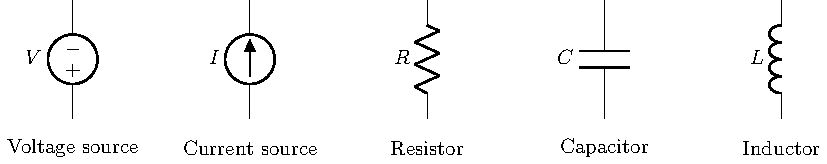
\includegraphics[width=\textwidth]{figures/ch02/fig02-01.pdf}
    \caption{Basic circuit elements: voltage source, current source, resistor, capacitor, and inductor.}
    \label{fig:02-01}
\end{figure}

\noindent\textbf{Independent Voltage source.} An Ideal voltage source provides a fixed voltage $V$ between its two terminals, and can provide any amount of current. Notice that the voltage $V$ can be fixed or time varying. For example, for a DC voltage source with $V = 5V$, the voltage across the two terminals will be $5V$ for all time. But for a time varying AC source, $V = 5 \sin \left( 100\pi t \right)$, the voltage across its terminal will vary with time. We will often drop the adjective "independent" when we are sure that the context is clear. We will look at dependent sources later, and we will always use the adjective "dependent" to refer to them.

\noindent \textbf{Independent Current source.} An ideal current source provides a fixed amount of current to flow throgh its terminals (out through one and in through the other), irrespective of the voltage across its terminals. Current sources can also be time-varying.

\noindent \textbf{Resistor.} A passive element where the current $i_R$ flowing through the element is proportional to the voltage $v_R$ across its terminals.
\[ v_R \propto i_R \]
In the case of linear resistors, the proportionality factor is constant, resulting in Ohm's law,
\begin{equation}
    v_R = R \, i_R
    \label{eq:02-01}
\end{equation}

The units of $R$ are $V.A^{-1}$ or $Omhs \left( \Omega \right)$. $R$ in general is positive. The power absorbed by a resistor is given by the product of the voltage across it and the current flowing through it, 
\begin{equation}
    P = v_R \, i_R = i_R^2 \, R = \frac{v_R^2}{R}
    \label{eq:02-02}
\end{equation}
This power is dissipated as heat by the resistor. Note that the power absorbed by a resistor is always positive, since $R$ is positive.

We will later see non-linear resistors, where the resistance varies as a function of the applied votlage, temperature and other factors. 

\noindent \textbf{Capacitor.} A capacitor is another passive element with the following voltage current relationship.
\begin{equation}
    i_C = C \frac{d v_C}{dt}
    \label{eq:02-03}
\end{equation}

The current $i_C$ through the capacitor is proportional to the rate of change of voltage across its terminals $v_C$. The proportionality factor is called the capacitance $C$, and has units of $F$ (Farads) or $C \cdot V^{-1}$. The voltage across the capacitor at any given time is proportional to the integral of the current flowing through it or the charge stored in the capacitor. The voltage across the capacitor is given by
\begin{equation}
    v_C = \frac{q}{C} = \frac{1}{C}\int i_C \, dt
    \label{eq:02-04}
\end{equation}

The instantaneous power absorbed by the capacitor is given by,
\begin{equation}
    P = v_C \, i_C = C \, v_C \frac{d v_C}{dt}
    \label{eq:02-05}
\end{equation}

The power absorbed by the capacitor can be positive or negative, depending on the direction of current flow. If the current is flowing into the capacitor, then the voltage across it is increasing, and the power absorbed is positive. If the current is flowing out of the capacitor, then the voltage across it is decreasing, and the power absorbed is negative. A capacitor stores energy in the form of electric field between its plates. The energy stored in a capacitor at any given time depends on the charge stored in it, and is given by,
\begin{equation}
    E = \frac{1}{2}  C \, v_C^2
    \label{eq:02-06}
\end{equation}

\noindent \textbf{Inductor.} An inductor is another passive element with the following voltage current relationship.
\begin{equation}
    v_L = L \frac{di_L}{dt}
    \label{eq:02-07}
\end{equation}

The voltage $v_L$ across the inductor is proportional to the rate of change of current $i_L$ flowing through it. The proportionality factor is called the inductance $L$, and has units of $H$ (Henries) or $V \cdot s \cdot A^{-1}$. The current through the inductor at any given time is proportional to the integral of the voltage across it. The current through the inductor is given by
\begin{equation}
    i_L = \frac{1}{L} \int v_L \, dt
    \label{eq:02-08}
\end{equation}

The instantaneous power absorbed by the inductor is given by,
\begin{equation}
    P = v_L \, i_L = L \, i_L \frac{di_L}{dt}
    \label{eq:02-09}
\end{equation}

The power absorbed by the inductor can be positive or negative, depending on the direction of current flow. If the current is flowing into the inductor, then the voltage across it is increasing, and the power absorbed is positive. If the current is flowing out of the inductor, then the voltage across it is decreasing, and the power absorbed is negative. An inductor stores energy in the form of magnetic field around it. The energy stored in an inductor at any given time depends on the current flowing through it, and is given by,
\begin{equation}
    E = \frac{1}{2}  L \, i_L^2
    \label{eq:02-10}
\end{equation}

\section{Kirchoff's Laws}
The five elements alone are not that interesting. But interesting things can be done by connecting these elements together in different ways to form an electrical circuit. The elements are connected together by wires, which are assumed to be perfect conductors, i.e. zero resistance. Consider the following circuit (Figure \ref{fig:02-02}),
\begin{figure}[t]
    \centering
    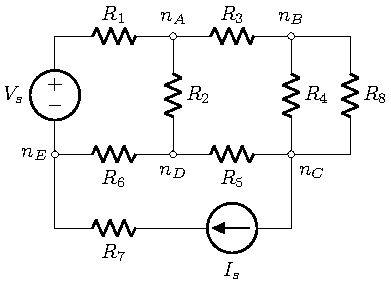
\includegraphics[width=0.5\textwidth]{figures/ch02/fig02-02.pdf}
    \caption{A simple electrical circuit with a voltage sourse, a current source, and a bunch of resistors.}
    \label{fig:02-02}
\end{figure}

How do we find out the voltages and currents in the circuit? Kirchoff's laws can be used for analysing such circuits, which are based on the conservation of charge and energy. The circuit in Figure \ref{fig:02-02} is a simple electrical circuit with a voltage source, a current source, and a bunch of resistors. The voltage source provides a fixed voltage $V_s$ between its two terminals, and the current source provides a fixed amount of current $I_s$ to flow through its terminals. The voltages and currents in the rest of the elements will be determined by Kirchoff's laws with the constraints imposed by the voltage and current sources. The two laws are:

\begin{enumerate}
    \item \textbf{Kirchoff's current law (KCL):} The sum of the currents entering a node is equal to the sum of the currents leaving the node. A \textit{node} is a point at which two or more circuit elements are connected together. In Figure \ref{fig:02-02}, $n_A$, $n_B$, $n_C$, $n_D$ and $n_E$ are examples of nodes where three elements are connected together. There are two other nodes in the circuit, can you identify them? 
    
    The sum of the currents at a node is equal to zero. This is based on the conservation of charge, and can be expressed mathematically as:
    \begin{equation}
        \sum_{i=1}^{n} i_i = 0
        \label{eq:02-11}
    \end{equation}
    where $i_i$ is the current flowing into or out of the node, and $n$ is the number of elements connected to the node. The current flowing into a node is positive, and the current flowing out of a node is negative.
    
    \item \textbf{Kirchoff's voltage law (KVL):} The sum of the voltages around a closed loop in a circuit is equal to zero. A \textit{closed loop} is a path in the circuit that starts and ends at the same node, and does not cross itself. In Figure \ref{fig:02-02}, the path starting from $n_A$, to $n_D$, to $n_B$, and back to $n_A$ is a closed path. This path includes the resistors $R_2$, $R_5$, $R_4$, and $R_3$. 
    
    This is based on the conservation of energy, and can be expressed mathematically as:
    \begin{equation}
        \sum_{i=1}^{n} v_i = 0
        \label{eq:02-12}
    \end{equation}
    where $v_i$ is the voltage across each element in the loop, and $n$ is the number of elements in the loop.

    The voltage across an element is positive if the current is flowing into the positive terminal of the element, and negative if the current is flowing out of the positive terminal of the element.
\end{enumerate}

Note that the two laws apply for any type of circuit element used in the circuits, independnet or dependent voltage/current sources, resistors, capacitors, inductors, either? two, three or four terminal elements.

\section{Series and Parallel Connections}
Two elements that share the same voltage across them between a given pair of nodes are said to be \textbf{parallel} to each other. In Figure~\ref{fig:02-02}, $R_4$ and $R_8$ are parallel to each other. In a single loop, two elements that share the same current are said to be in \textbf{series} with each other. In Figure~\ref{fig:02-02}, $V_s$ and $R_1$ are in series, $I_s$ and $R_7$ are in series.

\subsection{Resistors in series and parallel}
When $n$ resistors $R_1, R_2, \cdots R_n \geq 0$ are in series, these can be combined to an equivalent resistor with resistance $R_{eq}$ given by the following,
\begin{equation}
    R_{eq} = \sum_{i=1}^{n} R_i \implies R_{eq} \geq \max_{1 \leq i \leq n} R_i.
    \label{eq:02-13}
\end{equation}
Note that in a series connection the equivalent resistance is at least as large as the largest value of $R_1$ to $R_n$.

When $n$ resistors $R_1, R_2, \cdots R_n \geq 0$ are in parallel, these can be combined to an equivalent resistor with resistance $R_{eq}$ given by the following,
\begin{equation}
    \frac{1}{R_{eq}} = \sum_{i=1}^{n} \frac{1}{R_i} \implies R_{eq} = \frac{R_1R_2\cdots R_n}{R_1 + R_2 + \cdots + R_n} \implies R_{eq} \leq \min_{1 \leq i \leq n} R_i
    \label{eq:02-14}
\end{equation}
Note that in a parallel connection, the equivalent resistance cannot be larger than the smallest value of $R_1$ to $R_n$.

\subsection{Capacitors in series and parallel}
\noindent\textbf{Series connection} of $n$ capacitors $C_1, C_2, \cdots C_n \geq 0$
\begin{equation}
    C_{eq} = \frac{C_1C_2\cdots C_n}{C_1 + C_2 + \cdots + C_n}
    \label{eq:02-15}
\end{equation}

\noindent\textbf{Parallel connection} of $n$ capacitors $C_1, C_2, \cdots C_n \geq 0$
\begin{equation}
    C_{eq} = C_1 + C_2 + \cdots + C_n
    \label{eq:02-16}
\end{equation}

\subsection{Inductors in series and parallel}
\noindent\textbf{Series connection} of $n$ inductors $L_1, L_2, \cdots L_n \geq 0$
\begin{equation}
    L_{eq} = L_1 + L_2 + \cdots + L_n
    \label{eq:02-17}
\end{equation}

\noindent\textbf{Parallel connection} of $n$ inductors $L_1, L_2, \cdots L_n \geq 0$
\begin{equation}
    L_{eq} = \frac{L_1L_2\cdots L_n}{L_1 + L_2 + \cdots + L_n}
    \label{eq:02-18}
\end{equation}
Its left as an exercise for you to verify these expressions.

\noindent\textbf{What does the equivalent resistance actually mean?} The equivalent resistor with resistance $R_{eq}$ has the same voltage-current relationship as the individual elements in series or parallel connection. We can replace the series or parallel connection of the individual resistors $R_1$ to $R_n$ by a single resistor with value $R_{eq}$ without changing the volatage current relationships in the circuit. The same argument applies for equivalent capacitors and inductors.

\subsection{Voltage sources in series and parallel}
\noindent\textbf{Series connection} of $n$ voltage sources $V_1, V_2, \cdots V_n$ will result in an equivalent voltage source $V_{eq}$ given by
\begin{equation}
    V_{eq} = V_1 + V_2 + \cdots + V_n
    \label{eq:02-19}
\end{equation}
Voltage soruces should not be connected in parallel, as this will result in a short circuit. Ideally, an infinite current will flow through the connection, because the volatage sources force a potential difference between the two ends of the wire to be zero and it has zero resistance. Parallel connections are allowed only when the two sources have the same voltage and polarity.

\subsection{Current sources in series and parallel}
\noindent\textbf{Parallel connection} of $n$ current sources $I_1, I_2, \cdots I_n$ will
result in an equivalent current source $I_{eq}$ given by
\begin{equation}
    I_{eq} = I_1 + I_2 + \cdots + I_n
    \label{eq:02-20}
\end{equation}
Current sources should not be connected in series; series connections are allowed only when the two sources have the same current and polarity.

\section{Superposition Principle}
Linear approximations of circuits are often employed as first order approximations when analysing circuits. A linear ciruit is one that consists of linear passive elements, independent sources and linear dependent sources. Linear circuits follow the superposition principle, which states that the response of a linear circuit to a linear combination of inputs is equal to the corresponding linear comibnation of the responses to each input applied separately. Solving the following circuit (Figure~\ref{fig:02-03}) should make this concept clear.
\begin{figure}[t]
    \centering
    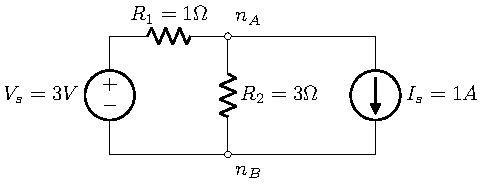
\includegraphics[width=0.65\textwidth]{figures/ch02/fig02-03.pdf}
    \caption{A simple circuit with two sources}
    \label{fig:02-03}
\end{figure}
For the circuit in Figure~\ref{fig:02-03}, perform the following calculation and compare your results.

\noindent\textbf{Step 1.} Solve for the voltage across and the current through the resistors $R_1$ and $R_2$; we will refer to these are $v_{R1}, i_{R1}$ and $v_{R2}, i_{R2}$, respectively. You should use both Kirchoff's current and voltages laws to compute these variables.

\noindent Let's now consider of the sources in the circuit seperately. This would mean making the source values ``zero''. This corresponds to two different operations on the circuit. Zeroing a voltage source corresponds to replacing it with a wire (a short circuit), while zeroing a current source corresponds to simple removing the current source (an open circuit). 

\noindent\textbf{Step 2.} Zero the voltage source $V_s$ and compute the voltages and currents associated with the two resistors. We will refer to these as $v_{R1,V_s=0}$, $v_{R2,V_s=0}$, $i_{R1,V_s=0}$, and $i_{R2,V_s=0}$.

\noindent\textbf{Step 3.} Zero the current source $I_s$ and compute the voltages and currents associated with the two resistors. We will refer to these as $v_{R1,I_s=0}$, $v_{R2,I_s=0}$, $i_{R1,I_s=0}$, and $i_{R2,I_s=0}$.

\noindent\textbf{Step 4.} For a linear circuit, shown in Figure~\ref{fig:02-03}, the following will always be true.
\begin{equation}
    \begin{split}
        v_{R1} &= v_{R1,V_s=0} + v_{R1,I_s=0}\\
        v_{R2} &= v_{R2,V_s=0} + v_{R2,I_s=0}\\
        i_{R1} &= i_{R1,V_s=0} + i_{R1,I_s=0}\\
        i_{R2} &= i_{R2,V_s=0} + i_{R2,I_s=0}\\
    \end{split}
    \label{eq:02-21}
\end{equation}

\noindent Let's assume that I am only interested in $i_{R2}$. Can I use $i_{R2,V_s=0}$ and $i_{R2,I_s=0}$ to compute the current $i_{R2}$ if $V_s = 1V$ and $I_s=-2A$? 

\section{Practical Voltage and Current Sources}
The independent voltage and current sources we have discussed so far are ``ideal'' sources. Practical or real sources do not behave like them - a battery cannot provide any amount of current for a load without any changes to the voltage across its terminals.

A good model of practical voltage source is an ideal voltage source $V_s$ in series with a \textit{internal}, \textit{source} or \textit{output} resistor $R_s$. And for a practical current source, it is an ideal current source $I_s$ in parallel with a resistor $R_s$. The voltage across the terminal of a voltage source as a function of the current drawn from it is depicted for an ideal and practical voltage source in Figure~\ref{fig:02-04}. For the ideal source (Figure~\ref{fig:02-04a}), the voltage $v_L$ is independent of the current $i_L$ drawn from it. For the practical voltage source (Figure~\ref{fig:02-04b}), the voltage across the terminals is a function of the current drawn from it,
\begin{equation}
    v_L = V_s - R_s \, i_L
    \label{eq:02-22}
\end{equation}
When $R_L = \infty$ ($i_L = 0$), the voltage across the terminals is equal to the voltage of the source $V_s$. This is maximum voltage the practical source can provide. This is also know as the \textit{open circuit voltage} $v_{oc}$ of the source. When $R_L = 0$ ($v_L = 0$), the current drawn from the source $i_L = \frac{V_s}{R_s}$. This is the maximum current the voltage source can provide. This is also known as the \textit{short circuit current} $i_{sc}$ of the source.

\begin{figure}[t]
    \centering
    \begin{subfigure}{0.48\textwidth}
        \centering
        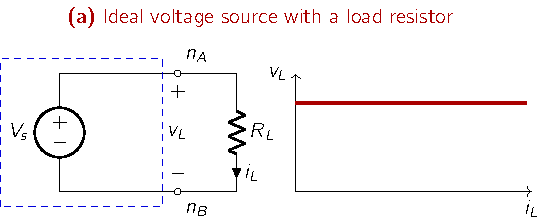
\includegraphics[width=\textwidth]{figures/ch02/fig02-04a.pdf}
        \caption{Ideal voltage source}
        \label{fig:02-04a}
    \end{subfigure}
    \hfill
    \begin{subfigure}{0.48\textwidth}
        \centering
        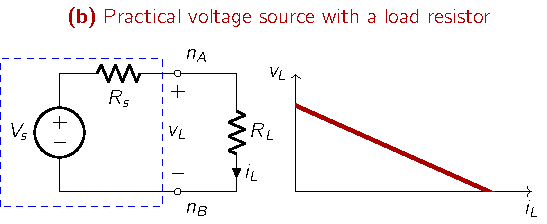
\includegraphics[width=\textwidth]{figures/ch02/fig02-04b.pdf}
        \caption{Practical voltage source with a load}
        \label{fig:02-04b}
    \end{subfigure}
    \caption{Comparison of the voltage-current relationship of an ideal and a practical voltage source.}
    \label{fig:02-04}
\end{figure}

\begin{boxedstuff}
    \begin{problem}
        Plot the voltage-current relationship of a practical current source with $I_s = 2A$ and $R_s = 10\Omega$. What are $v_{oc}$ and $i_{sc}$?
    \end{problem}
\end{boxedstuff}

\section{Thevenin's and Norton's Theorems}
Thevenin's and Norton's theorems are two important theorems in circuit theory that allow us to simplify complex circuits into simpler equivalent circuits. These theorems are based on the superposition principle, and can be used to analyze linear circuits with independent and dependent sources.

\noindent\textbf{Thevenin's Theorem.} Thevenin's theorem states that any linear circuit with independent and dependent sources can be replaced by an equivalent circuit with a single voltage source $V_{th}$ in series with a resistor $R_{th}$, connected to the load resistor $R_L$. 

\noindent\textbf{Norton's Theorem.} Norton's theorem states that any linear circuit with independent and dependent sources can be replaced by an equivalent circuit with a single current source $I_{N}$ in parallel with a resistor $R_{N}$, connected to the load resistor $R_L$.
\begin{figure}[t]
    \centering
    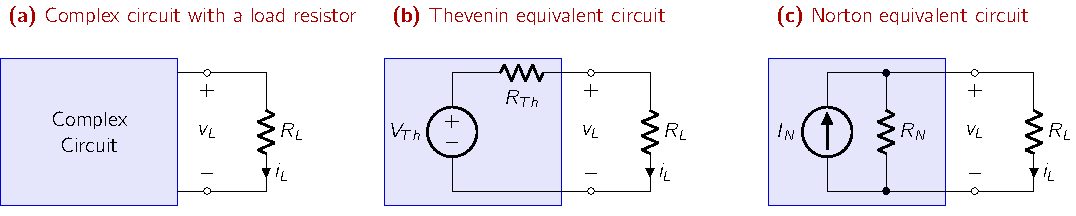
\includegraphics[width=\textwidth]{figures/ch02/fig02-05.pdf}
    \caption{Thevenin's and Norton's circuits for a complex linear circuit. The Thevenin and Norton equivalent circuits have the same voltage-current relationship for any load.}
    \label{fig:02-05}
\end{figure}

\noindent\textbf{Computing the Thevenin and Norton equivalent circuits.} The Thevenin and Norton equivalent circuits can be computed using the following steps:
\begin{enumerate}
    \item Remove the load resistor $R_L$ from the circuit.
    \item Compute the open circuit voltage $v_{oc}$ across the terminals of the load resistor. This is the Thevenin voltage $V_{th}$. This can be done using the superposition principle, where we zero all the independent sources except one and compute the open circuit voltage. The overall open circuit voltage is the sum of the open circuit voltages when all other sources are zeroed.
    \item Compute the short circuit current $i_{sc}$ through the terminals of the load resistor. This is the Norton current $I_{N}$. This too can be calculated using the superposition principle.
    \item Compute the Thevenin resistance $R_{th}$ by zeroing all independent sources in the circuit and computing the equivalent resistance seen from the terminals of the load resistor (without the load resistor). This is also equal to the Norton resistance $R_{N}$.
    \item The Thevenin and Norton equivalent circuits are then given by:
    \begin{equation}
        \begin{split}
            V_{th} &= v_{oc}\\
            I_{N} &= i_{sc}\\
            R_{th} &= R_{N}
        \end{split}
        \label{eq:02-23}
    \end{equation}
    \item The load resistor $R_L$ can be connected to either the Thevenin or Norton equivalent circuit, and the voltage and current across it can be computed using the voltage-current relationship of the equivalent circuit.
\end{enumerate}

\begin{boxedstuff}
    \begin{problem}
        Compute the Thevenin and Norton equivalent circuits for the circuit shown in Figur~\ref{fig:02-02} assuming the following as the load resistor: (a) $R_8$; (b) $R_2$; and (c) $R_7$.
    \end{problem}
\end{boxedstuff}

\section{Maximum Power Transfer Theorem}
The maximum power transfer theorem states that the maximum power is transferred to the load resistor $R_L$ when the load resistance is equal to the Thevenin resistance $R_{th}$ of the circuit. Consider the following circuit (Figure~\ref{fig:02-06}). The power absorbed by the load resistor $R_L$ is given by,
\begin{equation}
    P_{R_L} = \frac{R_L}{(R_{th} + R_L)^2} \, V_{th}^2
    \label{eq:02-24}
\end{equation}
Its easy to check that the optimal value of $R_L$ that maximizes the power absorbed by the load resistor is given by,
\begin{equation}
    \begin{split}
        R_L^* &= \arg\max_{R_L} \,\, \frac{R_L}{(R_{th} + R_L)^2} \, V_{th}^2 = R_{Th} \\
        P_L^* &= \max_{R_L} \,\, \frac{R_L}{(R_{th} + R_L)^2} \, V_{th}^2 = \frac{1}{4}\left(\frac{V_{Th}^2}{R_{Th}}\right)
    \end{split}
    \label{eq:02-25}
\end{equation}

\begin{figure}[t]
    \centering
    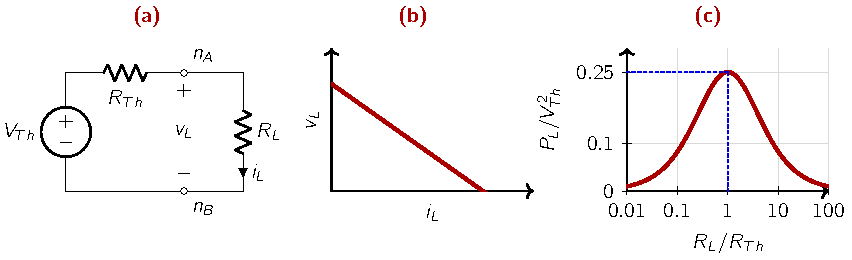
\includegraphics[width=\textwidth]{figures/ch02/fig02-06.pdf}
    \caption{Maximum power transfer theorem.}
    \label{fig:02-06}
\end{figure}

\begin{boxedstuff}
    \begin{problem}
        Prove the statements in Eq.~\ref{eq:02-25}. (\textit{Hint:} Use the first order condition for maximization of a continuous function.)
    \end{problem}
\end{boxedstuff}

\section{RC, RL, and RLC Circuits}
Unlike resistors, that neither remember the past values of its votlage or current, capacitors and indutors retain memory of the past current and past voltage, respectively. This can be easily seen from their respective voltage-current relationships given by Eq.~\ref{eq:02-03} and Eq.~\ref{eq:02-07}, respectively. 

\noindent\textbf{Capacitor:}
\begin{equation}
    i_C = C \frac{dv_C}{dt} \implies v_C\left(t\right) = \frac{1}{C}\int_{0}^{t} i_C\left(\tau\right) d\tau + v_C\left(0\right)
    \label{eq:02-26}
\end{equation} 
The instantaneous voltage across a capacitor contains some information about the past history the current that has flown through the capacitor. This voltage $v_C\left(t\right)$ is determined by the charge on the capacitor at time $t$. Note, that the voltage across the capacitor cannot change instantaneously, as this would require an infinite current to flow through the capacitor. Theoretically, however, an impulse (Dirac delta function) current applied to the capacitor can produce instantaneous change in the capacitor's voltage.

\noindent\textbf{Inductor:}
\begin{equation}
    v_L = L \frac{di_L}{dt} \implies i_L\left(t\right) = \frac{1}{L}\int_{0}^{t} v_L\left(\tau\right) d\tau + i_L\left(0\right)
    \label{eq:02-27}
\end{equation}
Similarly, the instantaneous current through the inductor contains some information about the history of voltage applied across the inductor. Current through an inductor cannot change instantaneously, as this would require an infinite voltage to be applied across the inductor. An impulse voltage applied to the inductor can produce instantaneous change in the inductor's current.

\noindent\textbf{RC Circuit.} Consider a simple RC circuit shown in Figure~\ref{fig:02-07a}. We can write Kirchoff's voltage law for the circuit as follows,
\begin{equation}
    RC \frac{d v_C}{dt} + v_C = V_s \implies v_C(t) = e^{-t/RC} \left[ v_{C}(0) + \int_0^t \frac{1}{RC} e^{\tau/RC} V_s(\tau)\, d\tau \right]
    \label{eq:02-28}
\end{equation}
The above euqation gives the general solution for the voltage across the capactior. We can derive all other variables of interest from $v_C$. The response to an impulse input, step input, sinusoidal input, or any arbitrary $V_s$ can be computed using the above equation. The response for a step input obtained using a fixed sources and a switch is given in Figure~\ref{fig:02-07a}. $RC$ is the time constant of the circuit, and is a measure of how fast the capacitor charges or discharges and it has the units of time.

\begin{figure}[t]
    \centering
    \begin{subfigure}{0.48\textwidth}
        \centering
        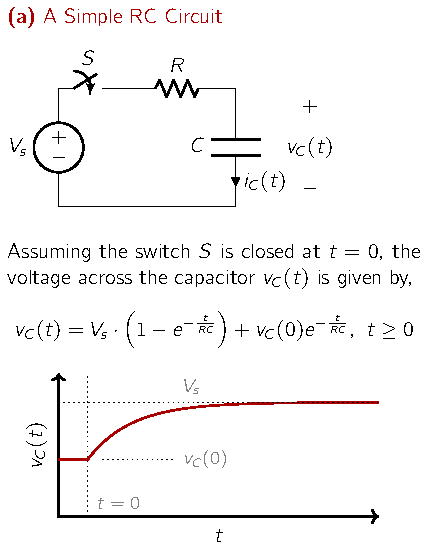
\includegraphics[width=\textwidth]{figures/ch02/fig02-07a.pdf}
        \caption{Ideal voltage source}
        \label{fig:02-07a}
    \end{subfigure}
    \hfill
    \begin{subfigure}{0.48\textwidth}
        \centering
        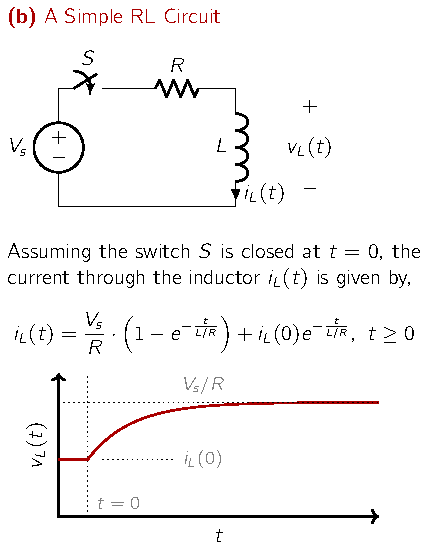
\includegraphics[width=\textwidth]{figures/ch02/fig02-07b.pdf}
        \caption{Practical voltage source with a load}
        \label{fig:02-07b}
    \end{subfigure}
    \caption{Simple RC and RL circuits and their transient responses.}
    \label{fig:02-07}
\end{figure}

Using Laplace transform to analyze the circuit, we can write the following expression for the voltage across the capacitor,
\begin{equation}
    V_C(s) = \frac{1}{sRC + 1} V_s(s) + \frac{v_C(0)}{sRC + 1}
    \label{eq:02-29}
\end{equation}
$V_C(s)$ and $V_s(s)$ are the Laplace transforms of $v_C(t)$ and $V_s(t)$. Replacing $s = j\omega$ will give us the frequency response of the system with $V_C(s)$ as the output and $V_s(s)$ as the input.

\noindent\textbf{RL Circuit.} Consider a simple RL circuit shown in Figure~\ref{fig:02-07b}. Kirchoff's voltage law for the circuit is as follows,
\begin{equation}
    \frac{L}{R} \frac{di_L}{dt} + i_L = \frac{1}{R}V_s \implies i_L(t) = e^{-tR/L} \left[ i_{L}(0) + \int_0^t \frac{1}{L} e^{\tau R/L} V_s(\tau)\, d\tau \right]
    \label{eq:02-30}
\end{equation}
The above euqation gives the general solution for the current through the inductor. The response to an impulse input, step input, sinusoidal input, or any arbitrary $V_s$ can be computed using the above equation. The response for a step input obtained using a fixed sources and a switch is given in Figure~\ref{fig:02-07a}. $\frac{L}{R}$ is the time constant of the circuit, and is a measure of how fast the current through the inductor can chamge; it has the units of time.

Similarly, applying the Laplace transform, we have,
\begin{equation}
    I_L(s) = \frac{1}{sL + R} V_s(s) + \frac{i_L(0)}{sL + R}
    \label{eq:02-31}
\end{equation}

\noindent\textbf{RLC Circuit.} Consider a simple series RLC circuit shown in Figure~\ref{fig:02-08}. Kirchoff's voltage law for the circuit is as follows,
\begin{equation}
    LC\frac{d^2 v_C}{dt^2} + RC \frac{d v_C}{dt} + v_C = V_s 
    \label{eq:02-32}
\end{equation}
\begin{figure}[t]
    \centering
    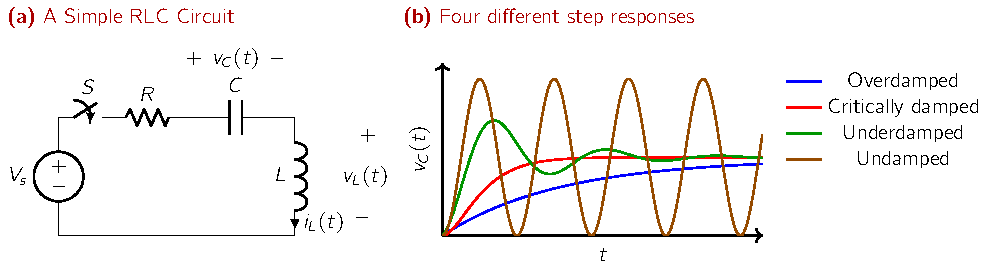
\includegraphics[width=\textwidth]{figures/ch02/fig02-08.pdf}
    \caption{A simple RLC circuit and the different respones of the circuit when the switch $S$ is closed at time $t = 0$, with  zero initial capacitor voltage and inductor current whent .}
    \label{fig:02-08}
\end{figure}
The response of the circuit when the switch is closed at $t=0$ is qualitatively different depending on the values of $R$, $L$ and $C$. This is better understood in the Laplace domain. The Laplace transform of the response $v_c(t)$ is given by,
\begin{equation}
    V_C(s) = \frac{V_s(s)}{LCs^2 + RCs + 1} + v_C(0)\frac{C\left(Ls + R\right)}{LCs^2 + RCs + 1} + i_L(0)\frac{RC}{LCs^2 + RCs + 1}
    \label{eq:02-33}
\end{equation}
Note that $i_L(0) = \frac{d v_C}{dt}(0)$. The denominator of the above equation is a second order polynomial in $s$, and thus the response of the circuit will depend on the roots of the polynomial. The four different responses are shown in Figure~\ref{fig:02-08}.

\section{Steady State Sinusoidal Analysis}
The previous subsection looked at the transient response of the some simple circuits involving $R$, $L$, and $C$. However, we are often interested in the steady state response of these circuits to sinusoidal excitations. This is because sinusoidal signals are eigenfunctions of linear systems, such as the linear circuits we have discussed so far. With sinusoidal excitations, all currents and voltages in the circuit will also be sinusoidal with the same frequency as the input excitations, althought with different amplitudes and phases. Complex numbers are used in this analysis for compact representation of ampltiude and phase of signals. 

For steady state frequency analysis for circuits involving $R$, $L$, and $C$, we extend the idea of resistance to impedance. Fourier transforms provide a natural way to analyze the steady state response of linear circuits to sinusoidal excitations. We first recast the voltage-current relationships of the circuit elements in the Fourier domain. 
\begin{equation}
    \begin{split}
        \textbf{Resistor:} \quad & v_R = R \, i_R \implies V_R\left(j\omega\right) = R \cdot I_R\left(j\omega\right)\\
        \textbf{Capacitor:} \quad & i_C = C\frac{d v_C}{dt} \, \implies V_C\left(j\omega\right) = \frac{1}{j\omega C} \cdot I\left(j\omega\right)\\
        \textbf{Inductor:} \quad & v_L = L \frac{d i_L}{dt} \implies V_L\left(j\omega\right) = j\omega L \cdot I_L\left(j \omega \right)
    \end{split}
    \label{eq:02-34}
\end{equation}

The Fourier transformed voltage-current relationships of the circuit elements look like Ohms law, with the concept of resistance extended to impedance. The impedance of a capacitor and inductor defined as the ratio of the Fourier transformed voltage to the Fourier transformed current. They are functions of the frequency of the voltage/current. The impedance of a resistor, capacitor, and inductor are given by,
\begin{equation}
    \begin{split}
        \textbf{Resistor:} \quad & Z_R = R\\
        \textbf{Capacitor:} \quad & Z_C = \frac{1}{j\omega C}\\
        \textbf{Inductor:} \quad & Z_L = j\omega L
    \end{split}
    \label{eq:02-35}
\end{equation}

\noindent\textbf{Equivalent Impedance.} The equivalent impedance of a circuit with impedances $Z_1, Z_2, \cdots Z_n$ in series is given by $Z_{eq} = Z_1 + Z_2 + \cdots + Z_n$. When the impedances $Z_1, Z_2, \cdots Z_n$ are in parallel, the equivalent impedances is given by $\frac{1}{Z_{eq}} = \frac{1}{Z_1} + \frac{1}{Z_2} + \cdots + \frac{1}{Z_n}$.

\noindent\textbf{Amplitude and phase modification by an impedance.} If a sinusoidal current excitation $i\left(t\right) = I_o \sin\left(\omega t\right)$ is passed through an impednace $Z$. Then the voltage across the impedance is given by,
\begin{equation}
    v\left(t\right) = \vert Z \vert I_o \sin\left(\omega t + \arg Z \right)
    \label{eq:02-36}
\end{equation}
The amplitude of the sinusoidal voltage is $\vert Z \vert I_o$, and the phase of the sinusoidal voltage is $\arg Z$, with respect to the current $i\left(t\right)$. 

\section{Exercise}
\vspace{-0.5cm}
\begin{center}
    \rule{\textwidth}{1pt}
\end{center}

\begin{enumerate}
    \item Plot the current through a resistor $R = 10\Omega$, capacitor $C = 5\mu F$, and inductor $L = 2mH$ for the following voltage inputs.
    \begin{figure}[h]
        \centering
        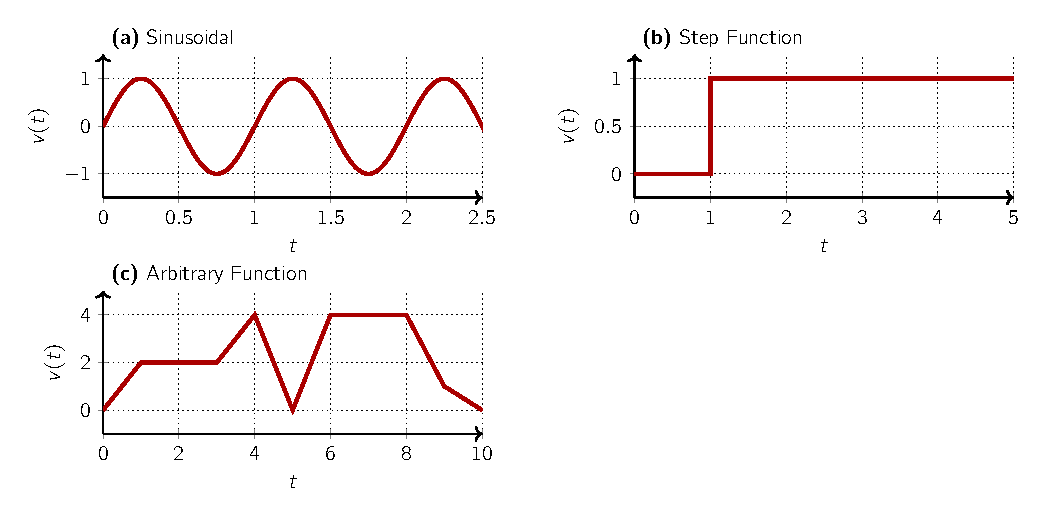
\includegraphics[width=\textwidth]{figures/ch02/ex02-01.pdf}
        \caption{[Exercise 1] Voltage inputs applied to a resistor, capacitor, or an inductor. The units of voltage are in volts, and the time is in seconds.}
        \label{fig:ex02-01}
    \end{figure}
    
    \item Find the Thevenin and Norton equivalent circuits of the following circuits (Figure~\ref{fig:ex02-02}). Note that one of the problems has a dependent source. Dependent sourcrs are voltage or current sources (diamond shaped elements), whose voltage or current, respectively, depend on the voltage or current across another element in the circuit.
    \begin{figure}[h]
        \centering
        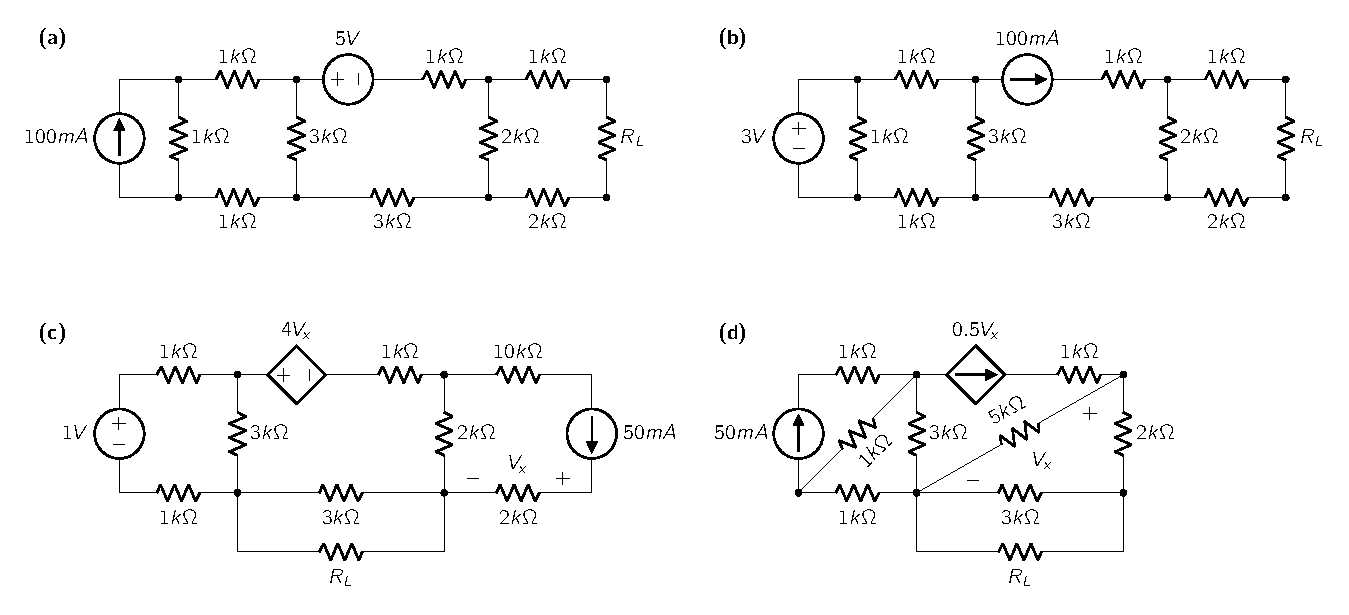
\includegraphics[width=\textwidth]{figures/ch02/ex02-02.pdf}
        \caption{[Exercise 2] Find the equivalent impedance of the circuit.}
        \label{fig:ex02-02}
    \end{figure}
    
    \item A certain red LED has a maximum current rating of $35 mA$, and if this value is exceeded, overheating and catastrophic failure will result. The resistance of the LED is a nonlinear function of its current, but the manufacturer warrants a minimum resistance of $47 \Omega$ and a maximum resistance of $117 \Omega$. Only $9 V$ batteries are available to power the LED. Design a suitable circuit to deliver the maximum power possible to the LED without damaging it. Use only combinations of the standard resistor values. (\textit{This problem is from Engineering Circuit Analysis by Hayt Jr. et al.})
    
    \item The load resistor in Figure~\ref{fig:ex02-03} can safely dissipate up to $1W$ before overheating and bursting into flame. The lamp can be treated as a $10.6\Omega$ resistor if less than $1A$ flows through it and a $15\Omega$ resistor if more than $1A$ flows through it. What is the maximum permissible value of $I_s$? Verify your answer with an appropriate computer simulation. (\textit{This problem is from Engineering Circuit Analysis by Hayt Jr. et al.})
    \begin{figure}[h]
        \centering
        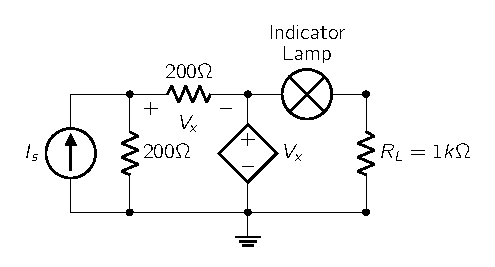
\includegraphics[width=0.65\textwidth]{figures/ch02/ex02-03.pdf}
        \caption{[Exercise 4]Find the equivalent impedance of the circuit.}
        \label{fig:ex02-03}
    \end{figure}
    
    \item In the following circuit (Figure~\ref{fig:ex02-04}), find the voltage across the capacitors $C_1$ and $C_2$. The single pole double throw swtich $S$ is connected to the top terminal before time $t=0$. At time $t=0$, swtich is flipped to the bottom terminal.  Assume that before time $t=0$, the voltage across the capacitor $C_2$, $v_{C2} = 1V$. Draw the plot of the voltage across the capcitors $C_1$ and $C_2$ as function of time.
    \begin{figure}[h]
        \centering
        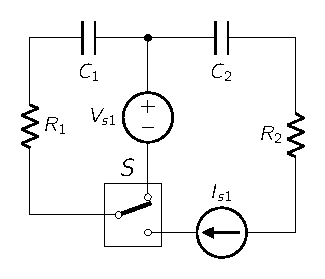
\includegraphics[width=0.35\textwidth]{figures/ch02/ex02-04.pdf}
        \caption{[Exercise 5]Find the equivalent impedance of the circuit.}
        \label{fig:ex02-04}
    \end{figure}
    
    \item Figure~\ref{fig:ex02-05} shows a voltage divider circuit with a sinusoidal voltage source $V_s\left(t\right) = 10 \sin\left(1000\pi t\right)$. The impedane $Z_1 = 3 + j4 \Omega$. What should the impedance $Z_2$ be if the the voltage across $Z_2$ has one-fourth the amplitude of $V_s$ and with a phase difference of $45\deg$?
    \begin{figure}[h]
        \centering
        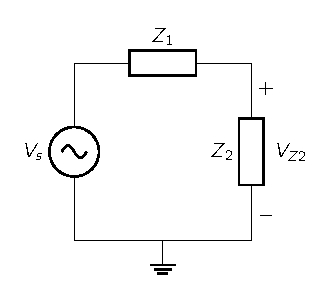
\includegraphics[width=0.35\textwidth]{figures/ch02/ex02-05.pdf}
        \caption{[Exercise 5]Find the equivalent impedance of the circuit.}
        \label{fig:ex02-05}
    \end{figure}
\end{enumerate}